% =============================================================================
% The CGAL Developers' Manual
% Chapter: Robustness Issues
% -----------------------------------------------------------------------------
% file   : robustness.tex
% authors: Stefan Schirra <stschirr@mpi-sb.mpg.de>
% -----------------------------------------------------------------------------
% $Id$
% $Date$
% =============================================================================

\chapter{Robustness Issues\label{chap:robustness}}

\ccChapterAuthor{Olivier Devillers ({\tt olivier.devillers@inria.fr})\\
Stefan Schirra
}
\ccIndexMainItemBegin{robustness}

Design and correctness proofs of geometric algorithms usually assume exact
arithmetic. Since imprecise calculations can cause wrong or, much worse,
mutually contradictory decisions in the control flow of an algorithm, many
implementations crash, or at best, compute garbage for some inputs. For
some applications the fraction of bad inputs compared to all possible
inputs is small, but for other applications this fraction is large.

\cgal\ has a layered design. The correctness of some components depends
on the correctness of the components that are used. Correctness of
a component means behaving according to its (mathematical) specification.
Simply speaking, the source of the robustness problem is that the default
hardware-supported arithmetic does not really fulfill the requirements of 
the algorithm, since it does not implement arithmetic on the real numbers.

Nevertheless, the generic implementation of the kernel primitives that are 
parameterized by the arithmetic (more precisely, by a number type)
assumes that the arithmetic plugged in does behave as real arithmetic.
The generic code does not and should not (otherwise it would slow down 
``exact'' number types) deal with any potential imprecision. There are
a number of (third-party provided) ``exact'' number types available for use
with \cgal, where ``exact'' means
that all decisions (comparison operations) are correct and that the
representation of the numbers allows for refinement to an arbitrary precision, 
if needed. 
Depending of the needed computations, a suitable exact number type
can be \ccc{Quotient<MP_float>} or \ccc{gmpq} if rational computations
are involved. 
If roots of polynomials are needed, then the solution is to use 
 \ccc{leda_real} provided by LEDA or \ccc{CORE::Expr} provided by CORE.


% Most notably, \ccc{leda_real}s provide easy-to-use adaptive 
% ``exact'' arithmetic for the basic operations and $\sqrt[k]{\ }$ operations.
% \lcTex{
% \begin{center}
%   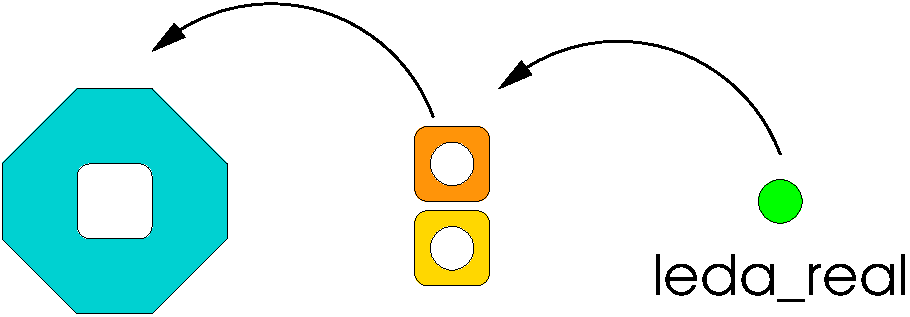
\includegraphics[width=8cm]{Developers_manual/fig/use_real}
% \end{center}
% }
% \lcRawHtml{
% <CENTER>
% <IMG BORDER=0 SRC="fig/use_real.gif"
%    ALT="Using LEDA reals for exact computation"><BR>
% </CENTER>
% }


\section{The role of predicates and constructions}
\cgal\ favors encapsulation of the basic arithmetic operations, the lowest
level in geometric computing, into units on a higher level, namely,
the level of geometric primitives, i.e., predicates and constructions. 
Here predicates are used in a generalized sense, i.e., not only primitives 
returning a Boolean value, but also primitives returning a value of 
some enumeration type, e.g.\ \ccc{CGAL::Sign}. So the value computed
by a predicate does not involve any numerical data. Basic constructions 
construct new primitive geometric objects that may involve newly computed
numerical data, i.e. that is not part of the input to the constructions. 
An example of such a basic constructions is computing the midpoint of
the straight line segment between two given points.
A special kind of constructions is selections. For selections, all the data
in the constructed objects was already part of the input. An example is
computing the lexicographically smaller point for two given points.

\cgal\ provides generic implementations of geometric primitives. These assume
``exact computation''. This may or may not work, depending on the actual
numerical input data. \cgal\ also provides\footnote{at present, for the 
dimension 2/3 Cartesian kernel(s) only.}
% The homogeneous counterpart still needs revision.}
specialization of the primitives
that (are still fairly generic and) guarantee exact predicate results and
much higher efficiency than exact number types like arbitrary precision
integers or rationals. The efficiency relies on the use of speedy 
floating-point arithmetic in order to filter out reliable floating-point 
computations. Interval arithmetic is largely used in such filter steps.
\ccIndexMainItemEnd{robustness}

\section{Requirements and recommendations}

Recommendations:
\begin{itemize}
\item Encapsulate basic arithmetic in predicates and constructions.
\item Use kernel primitives whenever possible. This allows you to use 
the kernel as a traits class for your algorithm or data structure.
\item If no appropriate kernel primitives are available, have a look at
Chapter \ref{chap:kernels} on how to proceed.
\end{itemize}

